\chapter{Introdução}
\label{cap:introducao}
Este capítulo apresenta o tema do trabalho, que visa analisar a complexidade crescente das aplicações web e a importância da escolha de uma estratégia de renderização. O estudo se aprofunda na avaliação das abordagens de \acrfull{csr} e \acrfull{ssr}, comparando sua eficácia para otimização de desempenho e experiência do usuário.


\section{Problema e contexto}
O crescimento acelerado da web e o aumento da complexidade das aplicações modernas impuseram novos desafios ao desenvolvimento e à entrega de conteúdos na internet. Com o crescimento exponencial da web, estima-se que aproximadamente 252 mil novos sites sejam desenvolvidos diariamente, demonstrando não apenas a rapidez com que aplicações são criadas, mas também a necessidade crescente de estratégias eficientes para otimização de desempenho e escalabilidade \cite{dataInternetUsage}. A escolha da abordagem de renderização tornou-se um fator determinante para a experiência do usuário e a escalabilidade dos sistemas. Inicialmente, os sites eram compostos por páginas estáticas, cujo conteúdo era carregado diretamente do servidor. Com a evolução das tecnologias frontend, novas abordagens surgiram, destacando-se \english{\acrfull{csr}} e \english{\acrfull{ssr}}. Cada uma dessas técnicas possui características específicas que influenciam diretamente o desempenho e a experiência do usuário.

A performance em websites é um fator determinante para o sucesso de qualquer aplicação web. O desempenho, frequentemente medido pelo tempo de carregamento das páginas, desempenha um papel fundamental na experiência do usuário e na taxa de conversão de visitantes \cite{webPerformance}. Uma página que carrega rapidamente proporciona uma navegação mais fluida, reduzindo a taxa de rejeição e aumentando a retenção de usuários. Além disso, o desempenho da página não se limita a impactar a experiência do usuário, mas também interfere diretamente no \english{\acrfull{seo}}, tornando-se um critério essencial de indexação e ranqueamento em plataformas como o Google \cite{google}.

Um exemplo notável de desafios enfrentados na escolha da estratégia de renderização ocorreu no \emph{Twitter}. Em 2010, a empresa lançou uma nova versão de sua plataforma, conhecida como New Twitter, que utilizava extensivamente a renderização no lado do cliente (\acrshort{csr}) para aprimorar a interatividade e a experiência do usuário. No entanto, essa abordagem resultou em problemas significativos de desempenho, especialmente para usuários com conexões de internet mais lentas ou dispositivos menos potentes. Além disso, a dependência intensa de JavaScript dificultou a indexação de conteúdo pelos mecanismos de busca, impactando negativamente a otimização para motores de busca (\acrshort{seo}) \cite{twitter}. Reconhecendo essas limitações, o Twitter decidiu retornar à renderização no lado do servidor (\acrshort{ssr}) em 2012, visando melhorar o desempenho e a acessibilidade de sua plataforma.

A arquitetura de frontend desempenha papel fundamental ao definir o fluxo de desenvolvimento e a escolha entre \acrshort{csr} e \acrshort{ssr}, sendo indispensável a adoção de um sistema modular e eficiente, capaz de ser mantido e escalado de forma sustentável \cite{frontendGodbolt}. Na abordagem \acrshort{csr}, a renderização ocorre diretamente no navegador do usuário, reduzindo a carga no servidor, mas exigindo mais processamento no cliente; já na \acrshort{ssr}, o conteúdo é gerado no servidor antes de ser enviado ao cliente, o que proporciona carregamento mais rápido e melhor desempenho em dispositivos menos potentes. A decisão entre essas estratégias está diretamente ligada à performance da aplicação e deve considerar fatores como tempo de carregamento, complexidade da página e número de requisições HTTP \cite{webPerformance}, já que diferentes abordagens afetam não apenas a experiência do usuário, mas também os custos operacionais e a infraestrutura necessária para suportar a aplicação.

\section{Justificativa}

Nos últimos anos, observou-se um crescimento expressivo na adoção de abordagens de renderização tanto no lado do cliente (\acrshort{csr}) quanto no lado do servidor (\acrshort{ssr}) em aplicações web, sobretudo quando comparadas a modelos tradicionais que utilizam apenas páginas estáticas ou \emph{templates} processados integralmente no servidor. Esse avanço deve-se, em grande parte, à busca contínua por melhor desempenho, experiências de usuário mais rápidas e dinâmicas, além da popularização de \emph{frameworks} e bibliotecas que simplificam a implementação dessas abordagens \cite{atori2024}.

Contudo, essas técnicas são frequentemente empregadas de maneira inadequada em muitos projetos, seja pela falta de entendimento de suas vantagens e limitações, seja por uma análise superficial das necessidades do produto. Um exemplo ilustrativo dessa realidade pode ser visto na experiência do \emph{Airbnb}, que optou por uma abordagem de \acrshort{ssr} com o intuito de melhorar o desempenho em dispositivos com recursos limitados e, sobretudo, otimizar a indexação de seu vasto catálogo de acomodações em mecanismos de busca \cite{neary2017}. Por outro lado, a equipe do \emph{Instagram} enfrentou desafios ao equilibrar o carregamento dinâmico de conteúdo no cliente com a necessidade de garantir uma experiência fluida aos usuários, levando-os a adotar soluções híbridas que envolvem tanto \acrshort{csr} quanto \acrshort{ssr} em diferentes partes da aplicação \cite{conner2019}.

Paralelamente a esses casos, identifica-se uma carência de estudos de caso reais que analisem de forma aprofundada o impacto da adoção de \acrshort{csr} e \acrshort{ssr}, principalmente no contexto nacional. Enquanto algumas publicações se concentram em apenas uma dessas abordagens, outras fornecem exemplos excessivamente simplificados, limitando a compreensão dos desafios técnicos e de negócios ao combinar essas estratégias em sistemas complexos.

Diante desse cenário, o presente trabalho se propõe a preencher essa lacuna por meio de uma análise detalhada e prática. Para isso, foi desenvolvido um estudo de caso focado em uma aplicação de notícias, implementada em duas versões funcionalmente idênticas: uma com \acrshort{csr} e outra com \acrshort{ssr}. Ao comparar diretamente os efeitos de cada abordagem no desempenho, na experiência do usuário, na otimização para \acrshort{seo} e na escalabilidade, espera-se fornecer subsídios concretos que possam orientar equipes de desenvolvimento e gestores na seleção da arquitetura de renderização mais adequada, auxiliando na construção de sistemas mais robustos e eficientes.

\section{Objetivos}
O objetivo geral deste trabalho de conclusão de curso é realizar uma análise comparativa detalhada entre \acrfull{csr}, aplicado em uma arquitetura \acrfull{spa}, e \acrfull{ssr}, associado a uma \acrfull{mpa}, materializada através do desenvolvimento e teste de um estudo de caso prático: uma aplicação de notícias implementada em ambas as arquiteturas. A análise busca avaliar, com base em dados empíricos, os efeitos de cada abordagem no desempenho, na experiência do usuário, na otimização do \acrfull{seo} e na escalabilidade de aplicações web modernas.

\subsection{Objetivos Específicos}
\begin{itemize}
\item Realizar uma análise comparativa do desempenho das abordagens \acrshort{csr} e \acrshort{ssr}, avaliando métricas focadas na experiência do usuário, como tempo de carregamento e interatividade, e o impacto no consumo de recursos do servidor (CPU e memória).

\item Identificar as principais limitações e desafios de cada arquitetura, especialmente no que se refere à otimização para mecanismos de busca (\acrshort{seo}) e à escalabilidade da aplicação.

\item Implementar o uso do sistema de controle de versão Git e da plataforma GitHub como instrumentos de gerenciamento do ciclo de desenvolvimento, documentando a organização de tarefas por meio de \textit{issues}, \textit{user stories} e quadros \textit{Kanban} e para garantir rastreabilidade, colaboração e reprodutibilidade do estudo de caso.
\end{itemize}

\item Apresentar recomendações práticas, baseadas nos dados coletados, para auxiliar equipes de desenvolvimento a decidir qual abordagem de renderização se alinha melhor aos requisitos de um projeto web.
\end{itemize}


% \section{Metodologia}
% Pode-se observar na \autoref{fig:metodo_recurso} as etapas de execução desta pesquisa. Inicialmente, o escopo é definido e o primeiro capítulo é elaborado, onde são apresentados o contexto do estudo, as justificativas e os objetivos a serem atingidos. Em seguida, constrói-se a fundamentação teórica, buscando fornecer uma base sólida para o desenvolvimento do estudo de caso por meio da discussão dos principais conceitos e tecnologias envolvidos.

% Posteriormente, realiza-se um mapeamento sistemático da literatura, cujo objetivo é identificar trabalhos similares, bem como lacunas no conhecimento, possibilitando a definição mais clara do escopo do estudo de caso. Além disso, essa fase permite levantar desafios, práticas e padrões comuns no uso de \acrshort{csr} e \acrshort{ssr}.

% Por fim, desenvolve-se um estudo de caso realista, no qual se descrevem requisitos, métodos e a arquitetura do sistema, bem como trechos de código ilustrativos da aplicação das técnicas. Nessa etapa, também são realizados testes de desempenho para avaliar o impacto das abordagens \acrshort{csr} e \acrshort{ssr} em termos de tempo de resposta, carga no servidor, experiência do usuário e otimização para \acrshort{seo}.

% Para concluir, elabora-se um relatório final que reúne análises quantitativas e qualitativas dos resultados, além de uma discussão sobre possíveis trabalhos futuros, desafios e benefícios do emprego de \acrshort{csr} e \acrshort{ssr} em aplicações web modernas.

% \begin{figure}[h!]
%     \centering
%     \caption{Etapas de desenvolvimento da pesquisa}
%     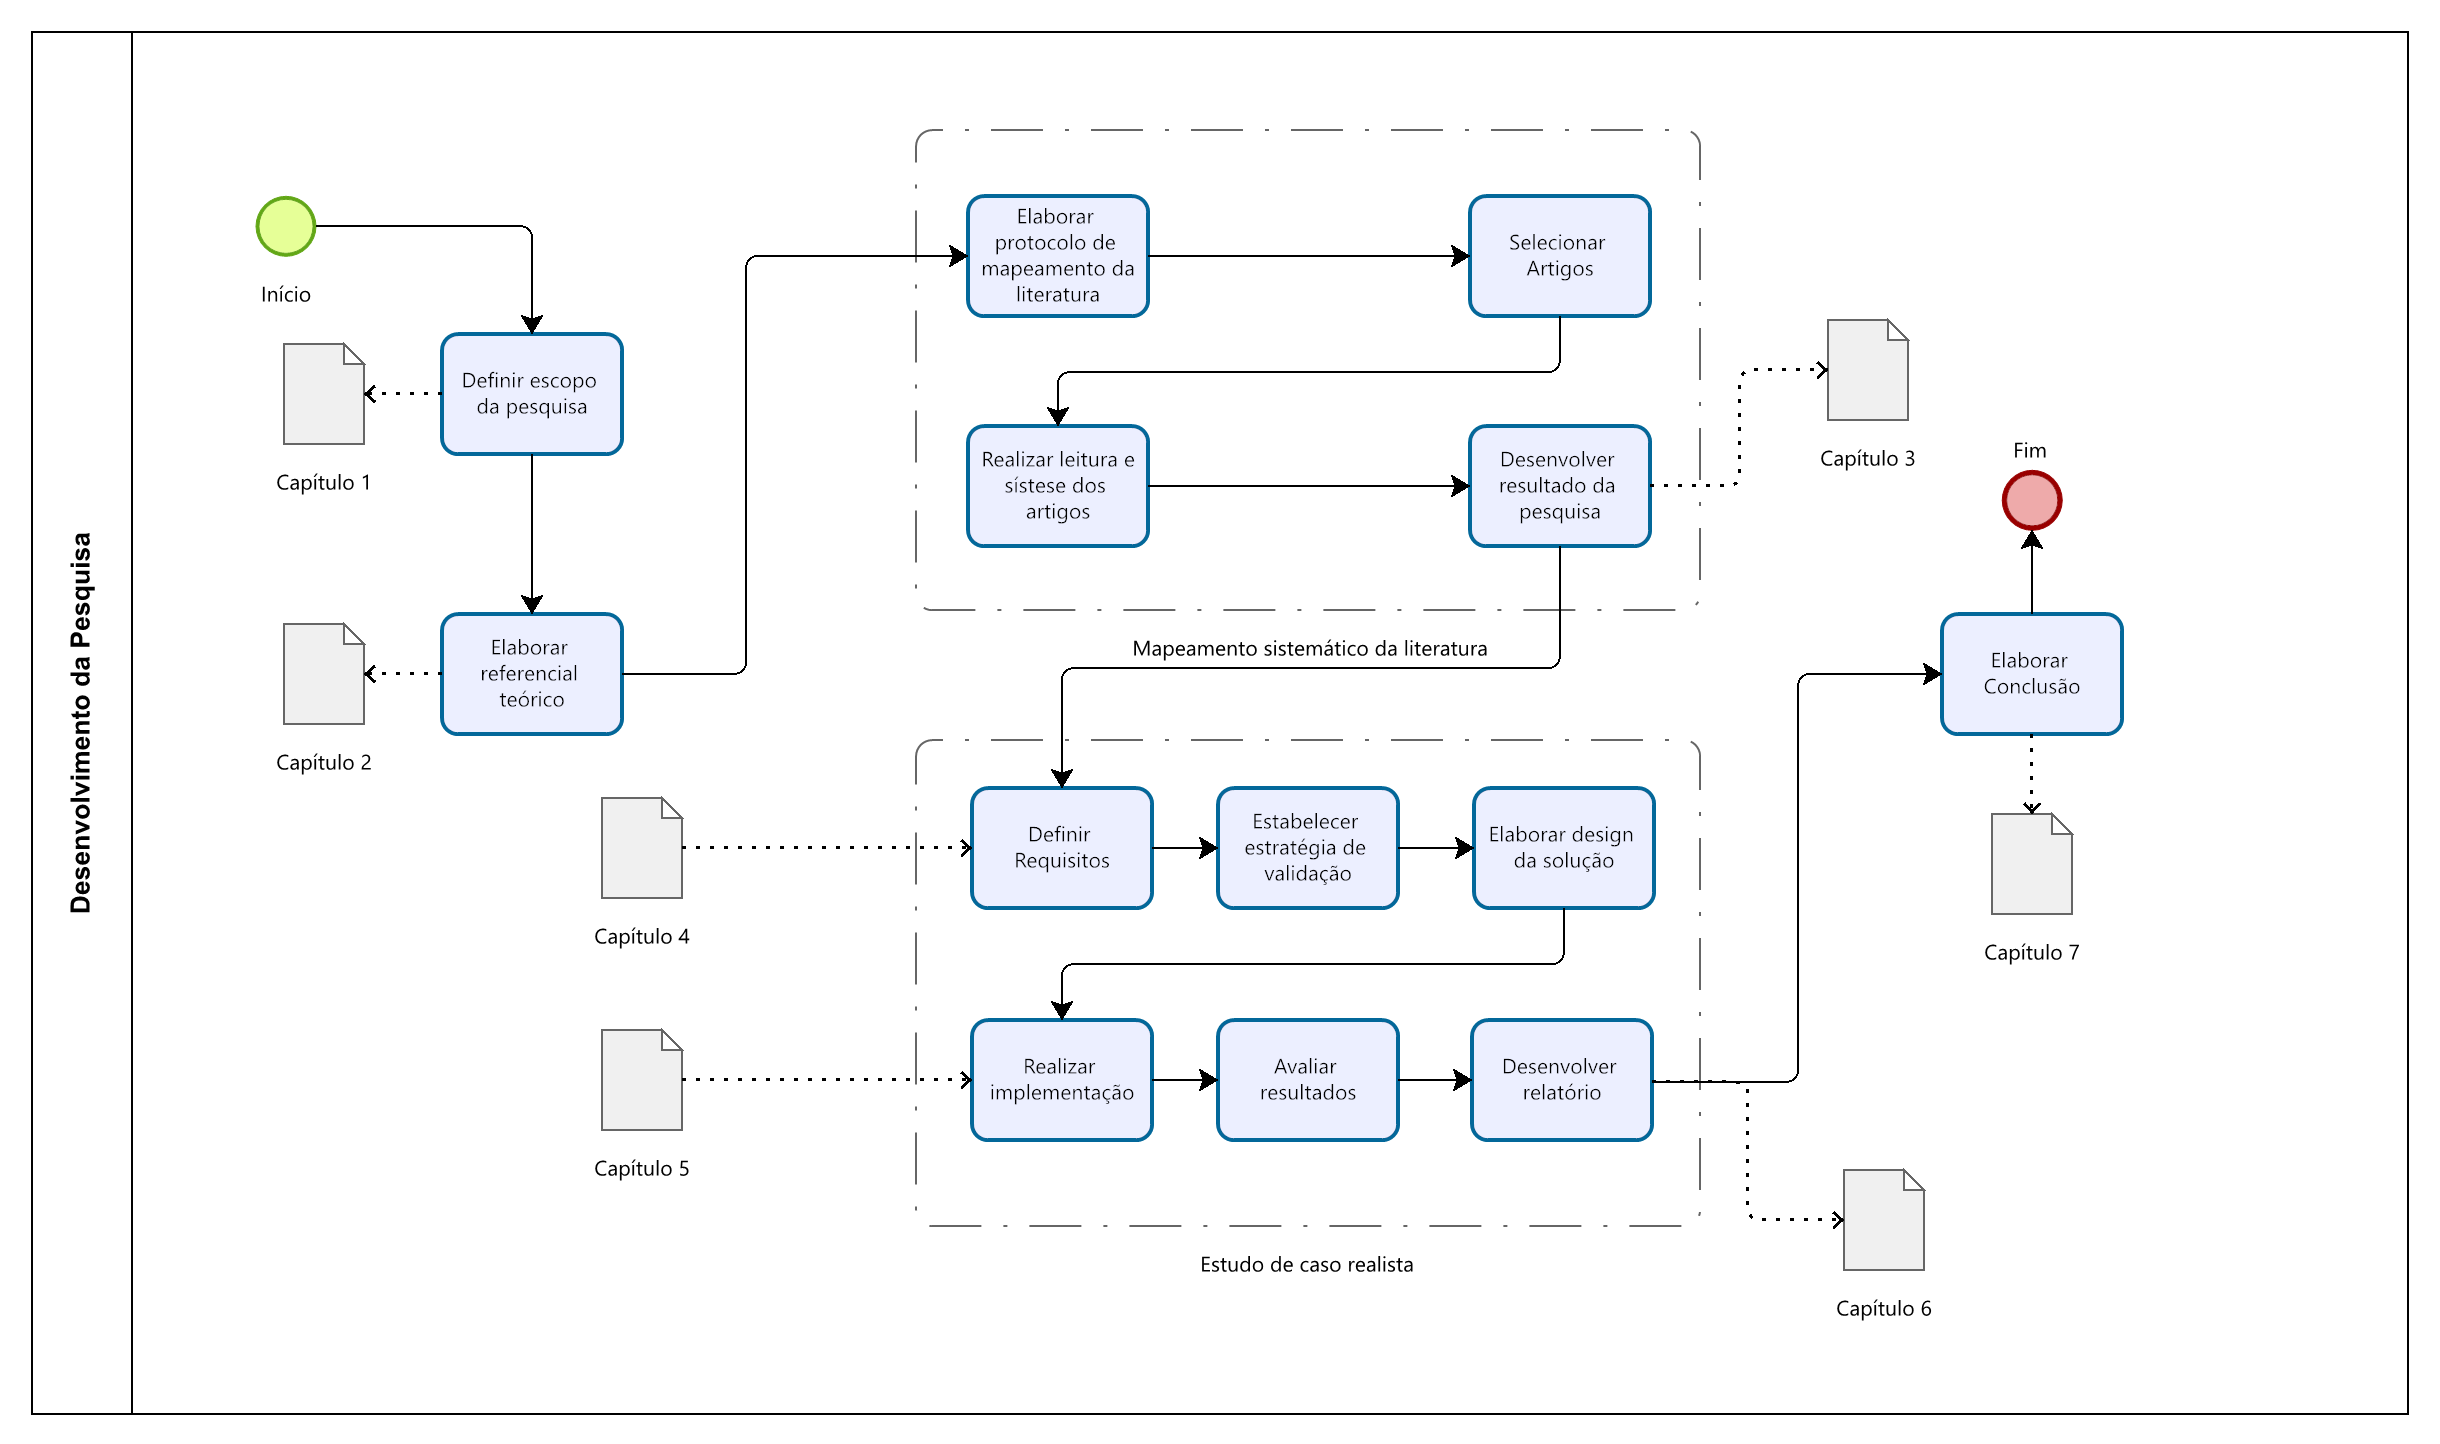
\includegraphics[width=0.9\textwidth]{media/bpmn_metodo_recurso.png}
%     \legend{Fonte: os autores}
%     \label{fig:metodo_recurso}
% \end{figure}

% \section{Estrutura do Trabalho}
% Este trabalho está dividido em sete capítulos. O \autoref{cap:introducao} expõe o contexto do estudo, as justificativas desta pesquisa e os objetivos a serem atingidos. O \autoref{cap:fundamentacao} apresenta conceitos fundamentais sobre \acrshort{csr} e \acrshort{ssr}, abordando suas principais características, vantagens e desafios. O \autoref{cap:trabalhos} expõe o protocolo e o resultado do mapeamento da literatura, analisando estudos relacionados e identificando lacunas no conhecimento sobre a adoção dessas abordagens. Da mesma forma, o \autoref{cap:estudo_caso1} descreve os requisitos, métodos e organização do estudo de caso. Em seguida, o \autoref{cap:estudo_caso1} apresenta o estudo de caso desenvolvido, incluindo o \english{design} do sistema e trechos de código chave da implementação. Posteriormente, o \autoref{cap:resultados} apresenta os resultados obtidos com a execução dos testes de desempenho, analisando métricas como tempo de resposta, consumo de recursos, impacto no \acrshort{seo} e experiência do usuário. Por fim, o \autoref{cap:conclusão} apresenta as conclusões obtidas com o desenvolvimento deste trabalho, destacando os principais achados, desafios e recomendações para a escolha entre \acrshort{csr} e \acrshort{ssr} em aplicações web modernas.